\documentclass{beamer}
\usepackage{pgfpages}
%\pgfpagesuselayout{4 on 1}[border shrink=5mm]

\usetheme{Singapore}
%\hypersetup{pdfpagemode=FullScreen}










\AtBeginSection{\frame{\sectionpage}}
\AtBeginSubsection{\frame{\subsectionpage}}
\AtBeginSubsubsection{\frame{\subsubsectionpage}}


\begin{document}





\section{Personal Identity}

%\frame{\begin{block}{There are three participants in this dialogue:}
%\begin{itemize}
%\item Gretchen Weirob, a philosophy professor
%\item Sam Miller, a chaplain and longtime friend of Gretchen’s.
%\item Dave Cohen, a former student of Gretchen’s
%\end{itemize}
%\end{block}
%\pause
%\begin{block}{The Challenge:}
%\begin{itemize}
%\item Gretchen, who is dying in the hospital, challenges Sam, a chaplain and religious believer, to prove to her that survival after the death of the body is possible.

%\item If Sam can do that, Gretchen says that she will be comforted. 

%\item Sam and Dave consider various arguments for thinking that persons can survive the death of the body, but Gretchen remains unconvinced.
%\end{itemize}
%\end{block}
%}

%\frame{\frametitle{Clarifying the Challenge}

%\begin{block}{Practice for the Pop Quizzes}
%What is the point of the example of the box of Kleenex? 
%\end{block}
%}

%\frame{\frametitle{Sample Answer}
%\pause
%\begin{itemize}
%\item[Sum up] The point is to draw attention to an ambiguity in the question whether one person is the same as another.%\pause
%\item[Elaborate] Gretchen survives only if after the death of her body there exists a person P such that Gretchen is the same as P.  But there is an ambiguity in the question whether  Gretchen is the same as P. It is this ambiguity that the discussion of the box of Kleenex is supposed to illustrate. Two boxes of Kleenex can be the same in the sense that they are qualitatively similar. Nevertheless, this does not make them numerically identical. \pause
%\item[Conclude] Gretchen survives only if there is a person P that she is numerically identical to. Her being qualitatively similar to P is not enough for her survival. 
%\end{itemize}
%
%}
%\frame{
%\begin{block}{Is survival \emph{possible}, could mean:}
%\begin{itemize}
%\item Is survival likely?
%\item Is survival compatible with the laws of physics? 
%\item Is survival metaphysically possible? 
%\pause
%\begin{itemize}
%\item Can we conceive of a coherent possible situation in which survival without the body occurred? \pause
%\end{itemize}
%\end{itemize}
%\end{block} 
%\begin{block}{Are square circles metaphysically possible?}
%\pause
%\begin{itemize}
%\item A square is a figure with four equal straight sides and four right angles.
%\item A circle is a plane figure whose boundary (the circumference) consists of points equidistant from a fixed point (the center).
%\item To coherently conceive of a square circle requires us to conceive of a figure with four equal straight sides and whose boundary consists of points equidistant from a fixed point. 
%\end{itemize}
%\end{block}
%}

%\frame{\frametitle{More Examples}
%\begin{itemize}
%\item Married bachelors are metaphysically impossible: Given what it is to be a bachelor, it is impossible to conceive of a bachelor who is married. 
%\item It is metaphysically possible that life on Earth did not come into being: Given what we know about the conditions required for life, we can imagine a scenario in which life never came about on Earth, e.g., a scenario in which there was no oxygen on Earth. 
%\item It is metaphysically possible that you did not come into being: there are scenarios in which the conditions required for your conception and birth were not satisfied. 
%\end{itemize}
%}
%


%\frame{\frametitle{Survival}
%\begin{block}{Two Considerations}
%\begin{itemize}
%\item G survives iff there is a person P at a time after her body has died  such that G is identical to P. \pause
%\item Survival must offer comfort of anticipation, e.g., it must make sense for G to look forward to P's pleasures and to fear P's pains. \pause
%\end{itemize}
%\end{block}
%\begin{block}{Conceiving Survival}
%\begin{itemize}
%\item Persons must be such that we can \emph{coherently} conceive a possible situation in which some person P exists yet 1) P does not have G's body, and 2) G = P
%\item What are we conceiving persons to be in such a situation? 
%\end{itemize}
%\end{block}
%}


\frame{
 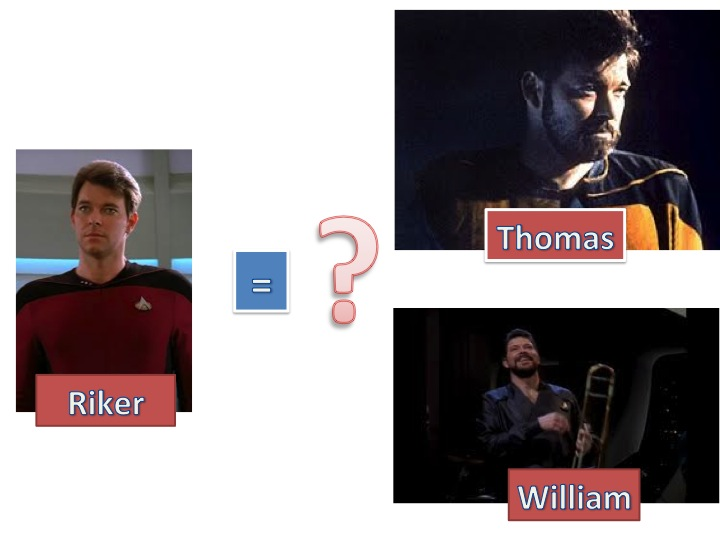
\includegraphics[width=\textwidth]{Slide1.jpg}
}






\frame{\frametitle{Remember!}
\begin{block}{Qualitative similarity \emph{vs.} numerical identity.} 
\begin{itemize} 
\item Two ginger bread men made by the same cookie cutter are qualitatively similar in several respects, e.g., they have the same shape, the same weight, the same colour, smell, and so on. But these are \emph{two} numerically distinct entities. 
\item Superman and Clark Kent are numerically identical, i.e., they are one and the same entity. If you want to count the number of entities in the room, you should only count Superman and Clark Kent once: Louis Lane makes a mistake when she counts them as two. 
\end{itemize}
\end{block}
}

%\frame{\frametitle{Possibility and Comfort}
%Consider tennis. If you play tennis with Serena Williams, you may lose. You may lose a lot! But suppose that you play her 100 times and win 1 game. This establishes that while it's improbable that you'll beat her on some occasion, it's still possible. This small possibility is enough to give you hope. Similarly, Gretchen will be comforted if surviving her bodily death, even if highly improbable, is still possible.
%}


\frame{\frametitle{What does personal identity consist in?}
Despite their qualitative differences, what is it about A that makes her the very same person as B?


 \begin{block}{Same Body Theory}
A person A at one time is identical to  a person B at a later time iff the body of A is identical to the body of B. \pause   
\end{block}
\begin{block}{Same Soul Theory}
A person A at one time is identical to  a person B at a later time iff the soul of A is identical to the soul of B. \pause
\end{block}
\begin{block}{Psychological Continuity Theory}
A person A at one time is identical to a person B
at a later time iff B is psychologically continuous with A.
 \end{block}
 }
 
\section{Sameness of Body}

\frame{
 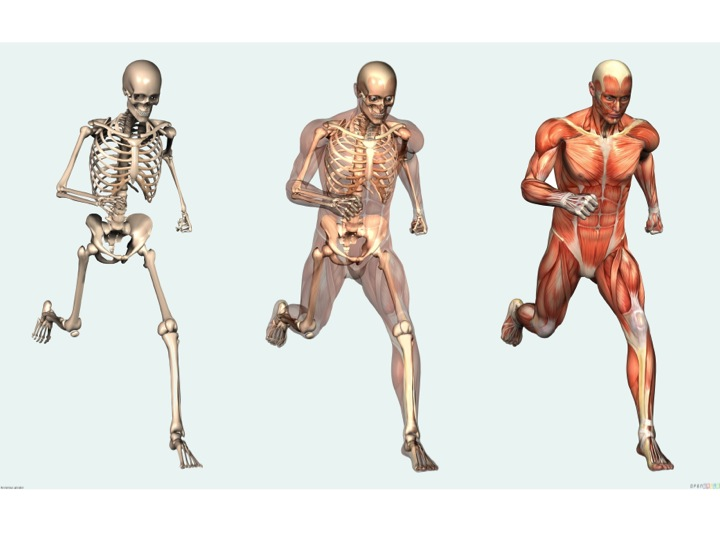
\includegraphics[width=\textwidth]{body.jpg}
}



\frame{\frametitle{Sameness of Body}
\begin{block}{Statement of Claim}
A person A at one time is identical to  a person B at a later time iff the body of A is identical to the body of B.
\end{block}
}

  \frame{
       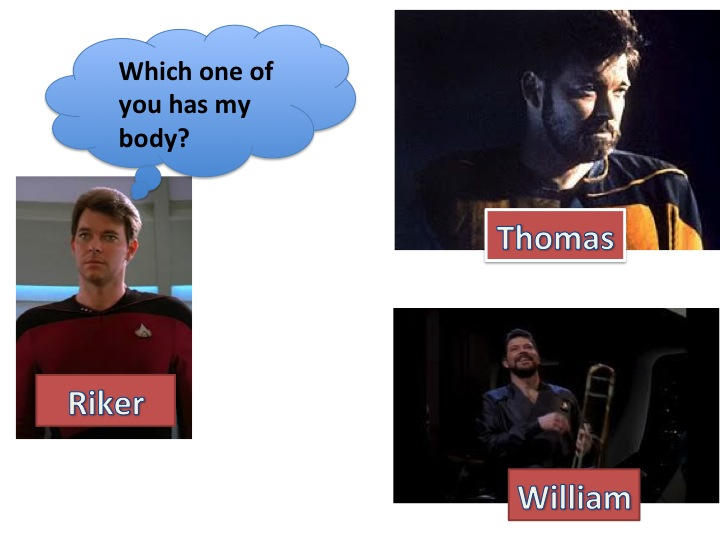
\includegraphics[width=\textwidth]{rikerb.jpg}
       }
 
 \frame{\frametitle{Discuss}

%\begin{block}{Does this meet Gretchen's challenge?}

%No! G's challenge is met only if there exists a person some time after her body has died who has her body. But the challenge assumes that her body has died. 
%\end{block}

\begin{block}{Virtues of this view?}
\begin{itemize}
\item We can perceive bodies. Thus the view explains how we are able to keep track and re-identify humans over time.
\end{itemize}
\end{block}
\begin{block}{Problems for this view?}
\begin{itemize}
\item Body swaps!
\end{itemize}
\end{block}
}
\frame{
 
\includegraphics[width=\textwidth]{freaky.jpg}
}


\section{Sameness of Soul} 

\frame{
       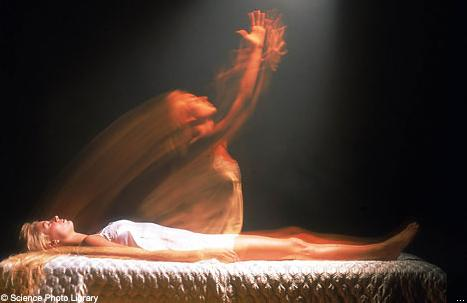
\includegraphics[width=\textwidth]{soul.jpg}
       }
       
       

 
\frame{\frametitle{Sameness of Soul}
\begin{block}{Statement of Claim}
A person A at one time is identical to  a person B at a later time iff the soul of A is identical to the soul of B.
\end{block}
}


 \frame{
 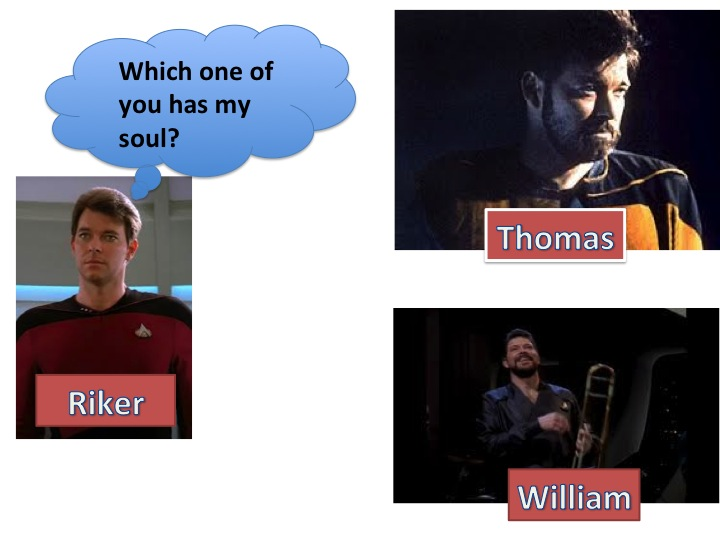
\includegraphics[width=\textwidth]{rikersoul.jpg}
 }
%\frame{\frametitle{Your Turn}
%\begin{itemize}
%\item What questions do you think must be answered to clarify the view? 
%\item Virtues of the view? 
%\item Problems for the view?
%\end{itemize}
%}

\frame{\frametitle{What is the soul?}
\begin{block}{Immaterial}
\begin{itemize}
\item Bodies are extended in 3-dimensions. 
\item Souls have no extension. 
\item There are simple bodies---the basic bits of matter---and complex bodies composed of matter. 
\item Souls are neither simple or complex bodies. 
\end{itemize}
\end{block}
\begin{block}{Seat of consciousness}
\begin{itemize}
\item For any thought and experience, there must be some entity which does the thinking and experiencing. 
\item Souls and not bodies are what think and experience. 
\end{itemize}
\end{block}
}

\frame{\frametitle{Immaterial}
 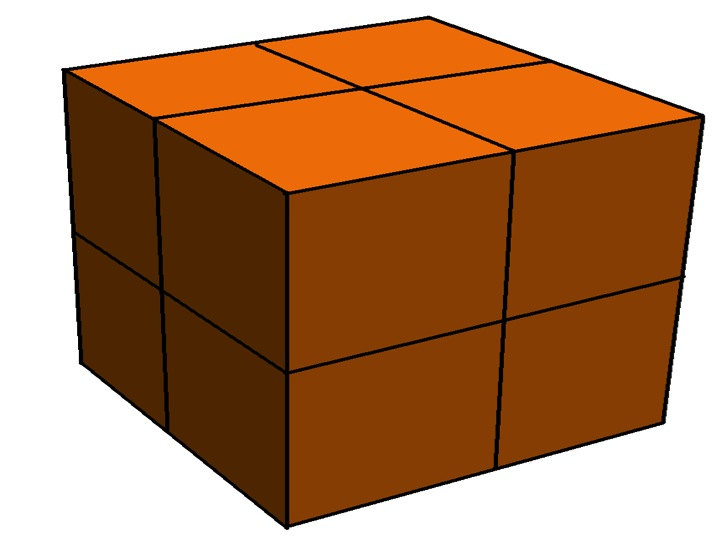
\includegraphics[width=\textwidth]{cube.jpg}
}
\frame{\frametitle{The Seat of Consciousness}
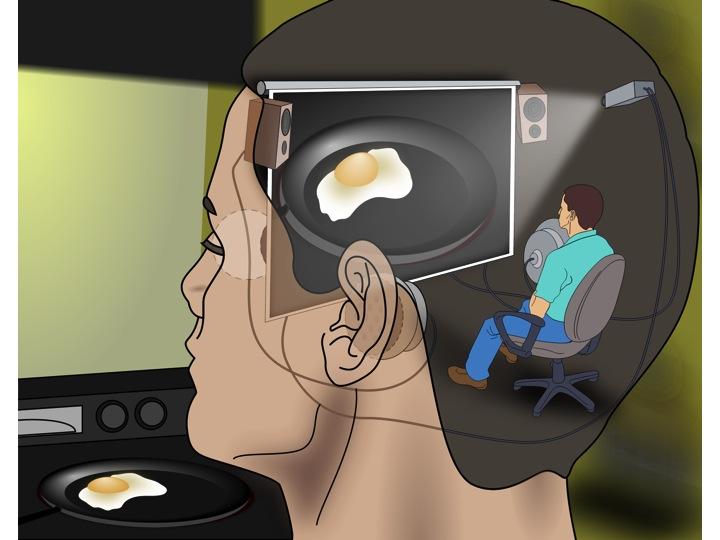
\includegraphics[width=\textwidth]{seat.jpg}
 }



\frame{\frametitle{Problems}
   \begin{itemize}
   \item  A person A at one time is identical to  a person B at a later time iff the soul of A is identical to the soul of B.
   \item  What evidence is there for this claim? \pause
   \item How could we know that the soul of A is identical to the soul of B?  \pause
   \begin{enumerate}
   \item  Direct experience? \pause
   \item Indirect experience: Same Body 
   \item Indirect experience: Same Psychology 
\end{enumerate}
\end{itemize}
   }

 \frame{\frametitle{Indirect Experience 1}
 \begin{block}{Claim}
 \begin{itemize}
 \item[B] Same body entails same soul. 
 \item We directly perceive bodies. 
 \item We indirectly perceive souls. \pause
\end{itemize}
\end{block}
%\begin{block}{Problems}
%\begin{itemize}
%\item[P1] If we can know that B is true, then B can be known either \emph{a posteriori} or \emph{a priori} \pause
%\item[P2] B cannot be known \emph{a posteriori}. \pause
%\item[P3] B cannot be known \emph{a priori}. \pause
%\item[C] Therefore, we cannot know that B is true. 
%\end{itemize}
%\end{block}
}

%\frame{\frametitle{Discussion of P2}
% 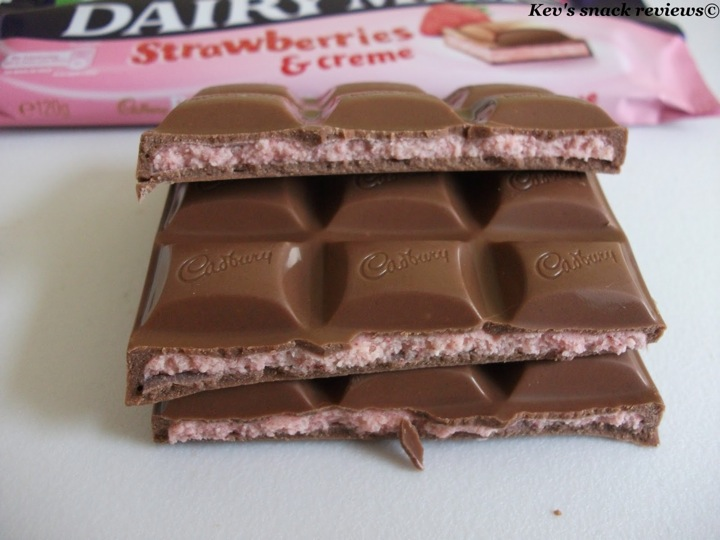
\includegraphics[width=\textwidth]{apost.jpg}

%}

% With the chocolate, I can test. My test involves me perceiving both the chocolate and the inside. We keep checking and we come to know that certain wrapper is associated with certain filling. But we can't check whether souls are associated with bodies. 

%\frame{\frametitle{Discussion of P3}

% 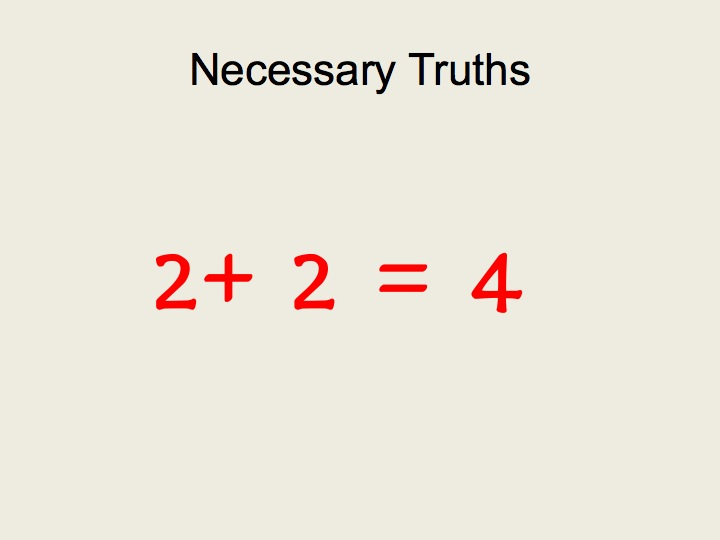
\includegraphics[width=\textwidth]{apr.jpg}
%}



\frame{\frametitle{Indirect Experience 2}
\begin{block}{Claim}
\begin{itemize}
\item[S] Same psychology entails same soul.  \pause
\item We can directly know that the psychology of A is the same as the psychology of B. \pause
\item Thus we can indirectly know that the soul of A is the same as the soul of B. \pause
\end{itemize}
\end{block}
%\begin{block}{Problems}
%\begin{itemize}
%\item[P1] If same psychology entailed same soul, then exemplification of psychological traits would be infallible evidence for sameness of soul.
%\item[P2] Exemplification of psychological traits are not infallible evidence for sameness of soul.
%\item[C] Same psychology does not entail same soul.
%\end{itemize}
%\end{block}
}

%\frame{\frametitle{Fallible vs. Infallible Evidence for Personal Identity}

% 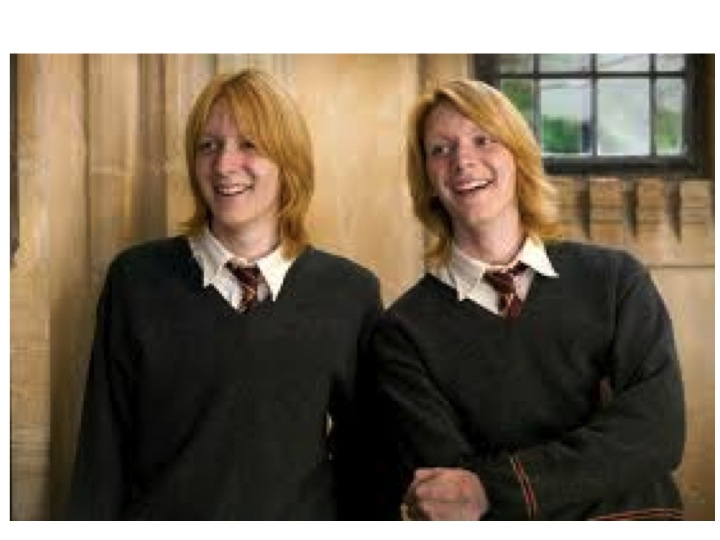
\includegraphics[width=\textwidth]{twins.jpg}
%}

\frame{
 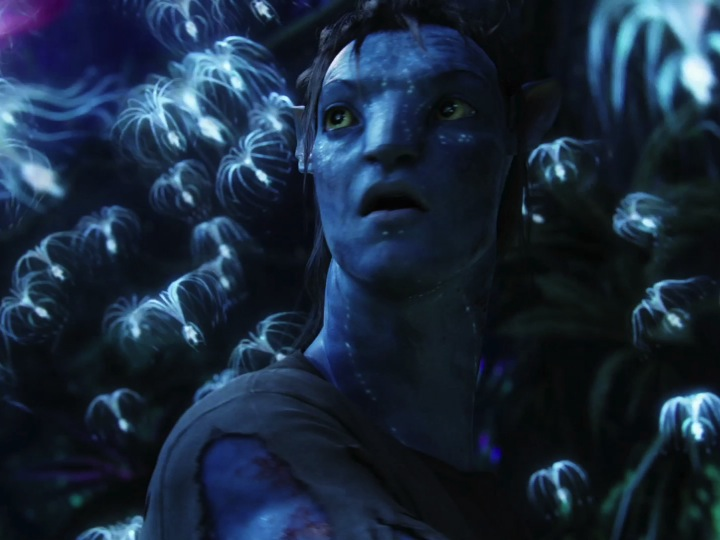
\includegraphics[width=\textwidth]{seeds.jpg}
}

\frame{\frametitle{Swapping Souls}
Consider a scenario in which 1) a series of souls flow into and out of the same body, and 2) that same body exhibits the same psychological traits.  If personal identity consists in sameness of soul, then there is a numerically distinct person every time a soul is exchanged. However, with every soul exchange there is no corresponding change in body or psychological traits. Thus same body does not entail same soul. Thus same psychology does not entail same soul.
}


\section{Memory \& Psychology}

\frame{\frametitle{Further Clarification of our Question}
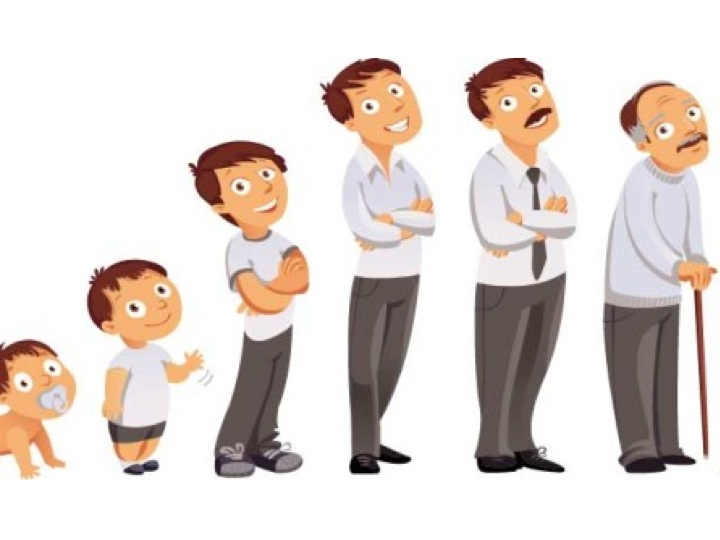
\includegraphics[width=\textwidth]{stages.jpg}
}

\frame{\frametitle{Appropriate Connection: Example}
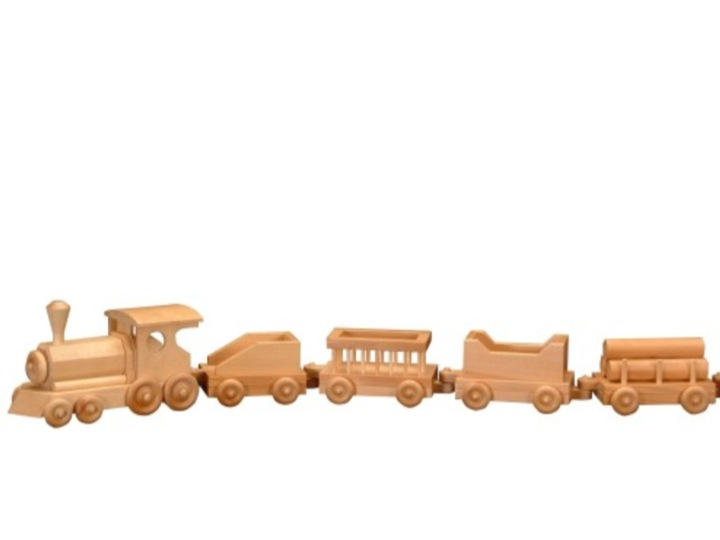
\includegraphics[width=\textwidth]{train.jpg}
}

\subsection{Version 1}

\frame{\frametitle{Memory Continuity}

A person A at one time is identical to a person B
at a later time iff B \emph{remembers} the \emph{experiences} that A has. 

}



\frame{\frametitle{Memory}


\begin{block}{Factual Memories} Memories that a particular event occurred. They can be shared by several people, e.g., many of us remember President Obama's inauguration.
\end{block}
\begin{block}{Personal Memories} Memories of having the experience of an event. They cannot be shared, e.g., only President Obama has the memory of \emph{being inaugurated} at his inauguration. 
\end{block}

}

\frame{
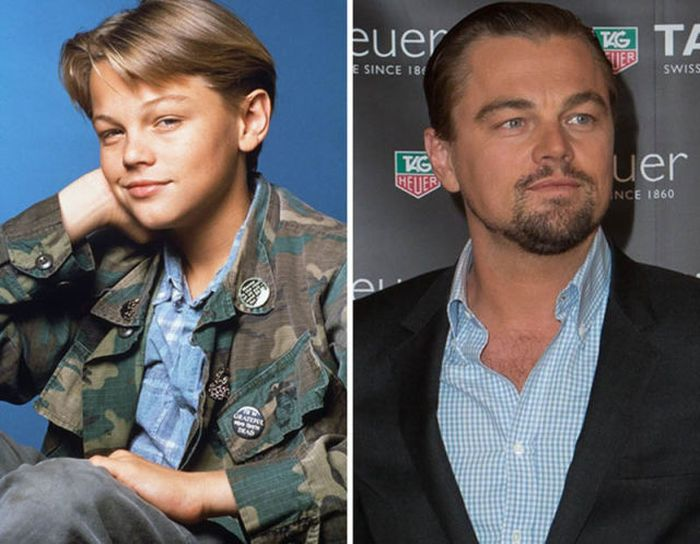
\includegraphics[width=\textwidth]{leo.jpg}
}
\frame{\frametitle{Objection}

\begin{itemize}
\item Allow `Rike' to be the 7 year old who will grow up to be Riker.
\begin{itemize}
\item[P1] Riker = Rike only if Riker remembers everything that Rike experenced. 
\item[P2] Riker does not remember what Rike ate for breakfast on the second day after his 7th birthday, though Rike certainly had the experience of eating something
\item[C] Riker $\neq$ Rike
\end{itemize}
\end{itemize}
}

\subsection*{Version 2}

\frame{\frametitle{Psychological Continuity-Version 2}

A person A at one time is identical to a person B
at a later time iff B is psychologically continuous with A.

\begin{block}{Psychological Continuity}
There is a chain of person-stages connected by
episodic memory.
\end{block}
}

\frame{\frametitle{Psychological Continuity}

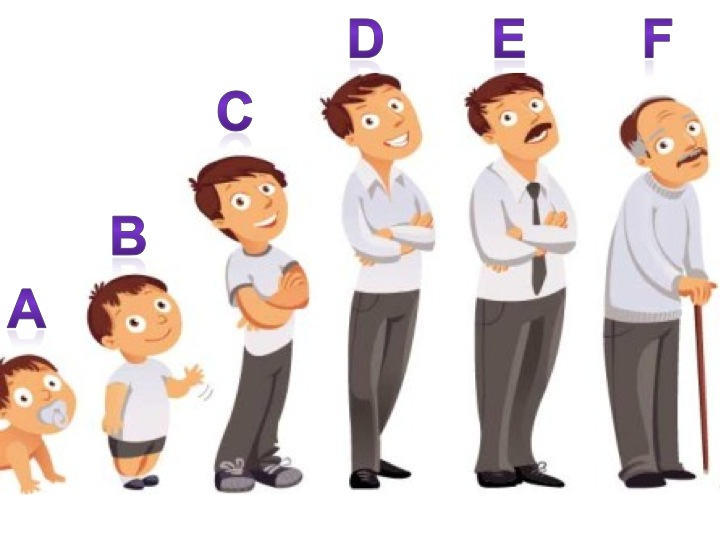
\includegraphics[width=\textwidth]{letters.jpg}

}
\frame{
\begin{itemize}
\item F remembers what E experienced.
\item E remembers what D experienced.
\item D remembers what C experienced.
\item C remembers what B experienced.
\item B remembers what A experienced.
\item Thus, A, B, C, D, E, and F are psychologically continuous with each other. 
\item Hence, they are all stages of the one very same person.
\end{itemize}
}

\frame{\frametitle{River Objection}
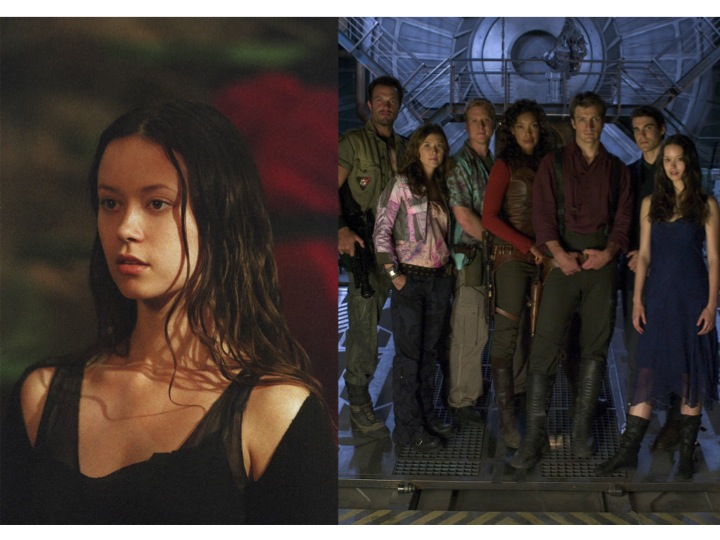
\includegraphics[width=\textwidth]{river.jpg}
}
\frame{\frametitle{Problem: Apparent vs Real Memory}
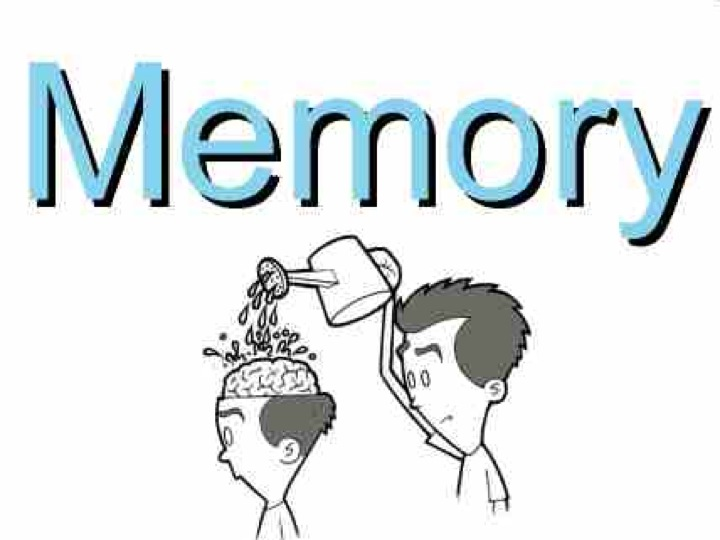
\includegraphics[width=\textwidth]{fake.jpg}
}

% false memory syndrome-false memories of traumatic experiences.
%Misinformation effect - experience that x is P. Someone tells you things about P and it changes your memory of x. 
% Rich false memories - not just distorted memories of what happened, memories of things which never happened. 
% 




\frame{

\begin{block}{I really remember X iff}
\begin{itemize}
\item I have an experience as though I
remember experiencing X.
\item I did experience X.
\end{itemize}
\end{block}

\begin{block}{I apparently remember X iff}
\begin{itemize}
\item I have an experience as though I remember experiencing X.
\item I did not experience X.
\end{itemize}
\end{block}
}


\frame{\frametitle{Distinguishing Real vs. Apparent Memories: Attempt 1}

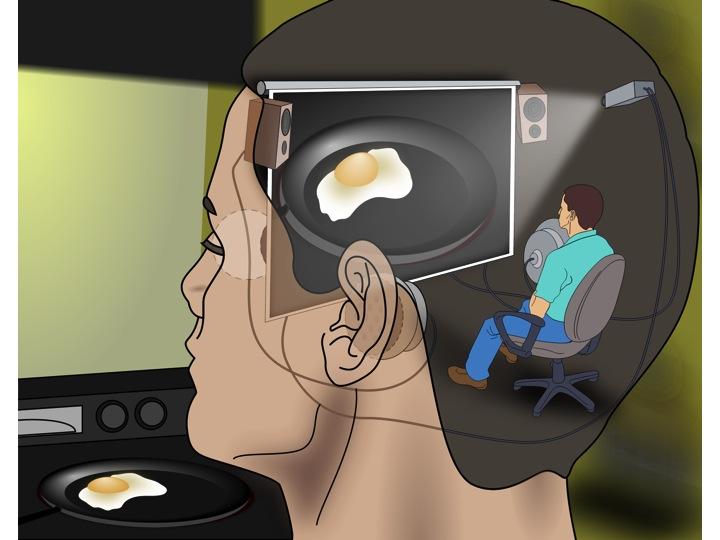
\includegraphics[width=\textwidth]{seat.jpg}

}

\frame{\frametitle{Internal Differences}

\begin{itemize}
\item[P1] If I could perceive a qualitative difference between a real and an apparent memory of X, then this qualitative difference would distinguish the real and apparent memory of X.
\item[P2] I can perceive no qualitative difference between a real and an apparent memory of X.
\item[C] No qualitative difference distinguishes real and apparent memories of X. 
\end{itemize}

}

\frame{\frametitle{Distinguishing Real vs. Apparent Memories: Attempt 2}

\begin{block}{Suggestion:}
If two persons A and B both have an experience as though they remember the experiences of some person P, then the memory of A (or B) is real and not apparent only if A (or B) is identical to P. 
\end{block}
\begin{block}{The problems is that it is circular to make both claims:}
\begin{enumerate}
\item A = P only if A really remembers what P experiences. 
\item A really remembers what P experiences only if A = P. 
\end{enumerate}
\end{block}
}

\frame{\frametitle{Circular Reasoning}

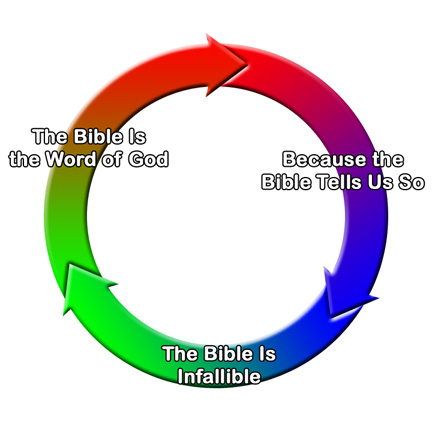
\includegraphics[width=\textwidth, height=\textheight]{circularity.jpg}

}

\frame{\frametitle{Distinguishing Real vs. Apparent Memories: Attempt 3}

\begin{block}{Suggestion}
\begin{itemize}
\item A real memory is one that was caused in the right way.
\item An apparent memory is one that was not caused in the right way, e.g. hypnosis, implantation, etc.\pause
\end{itemize}
\end{block}
\begin{block}{Problem-Duplicates!}
\begin{itemize}
\item[P1] Two persons A and B both have memories of what P experienced that were caused in the right way.
\item[P2] A $\neq$ B.
\item[C] Having memories caused in the right way is not sufficient for personal identity.
\end{itemize}
\end{block}
}
\frame{\frametitle{Riker Objection}
 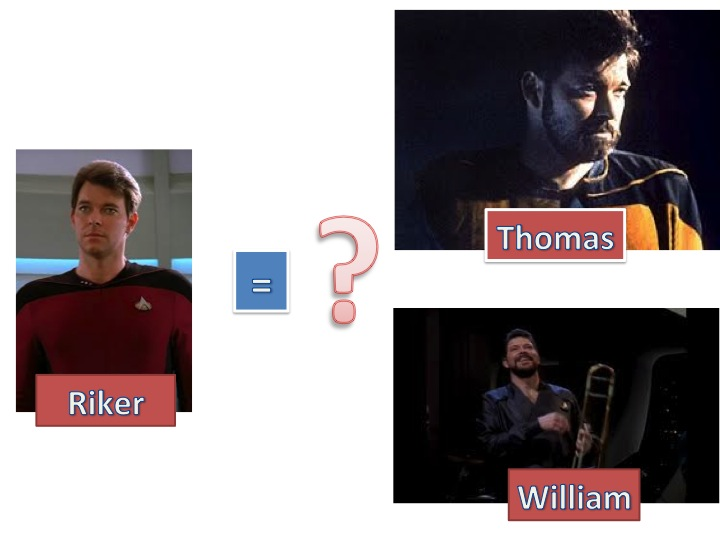
\includegraphics[width=\textwidth]{Slide1.jpg}
}

\end{document}
















 

